
\subsubsection{A. Score Distributions at Epoch 5}

\begin{figure}[htbp]
\centering
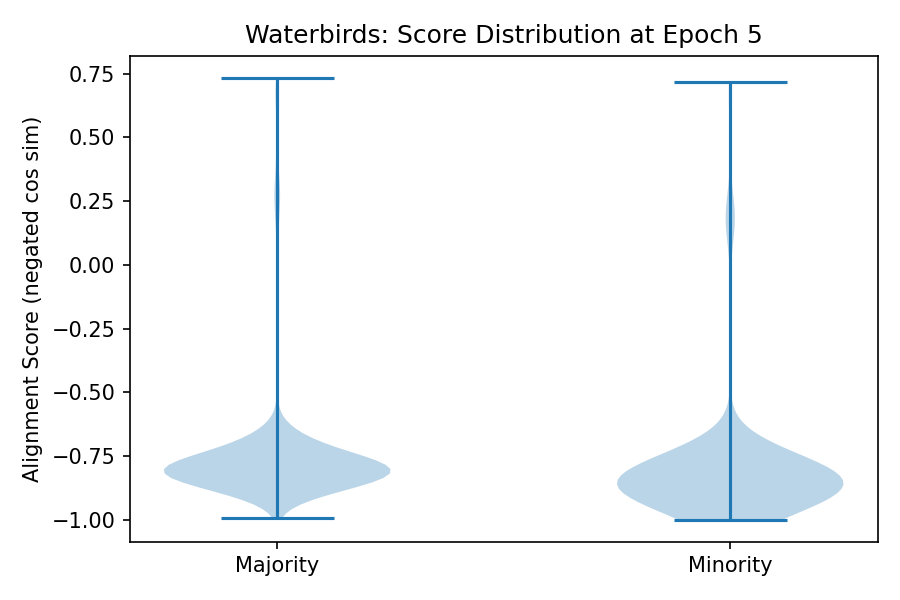
\includegraphics[width=\columnwidth]{figures/score_distribution_epoch5_waterbirds.png}
\caption{Score distributions at epoch 5 by group, Waterbirds}
\label{fig:score_distribution_epoch5_waterbirds}
\end{figure}

\textbf{Figure 4:} Alignment score ($a_i$) and per-sample loss distributions by group on Waterbirds at epoch 5, displayed as overlaid kernel density estimates. The minority groups (landbird-on-water, waterbird-on-land; group IDs {1, 2}) are shifted toward \textit{lower} $a_i$ values relative to majority --- i.e., higher raw cosine similarity with the batch mean --- confirming the inversion: minority samples appear more aligned with the batch mean, not less. Loss distributions in the same figure show clean minority/majority separation consistent with loss ROC-AUC = 0.854 at epoch 5. Source: \texttt{h-e1/figures/score\textbackslash \_distribution\textbackslash \_epoch5\textbackslash \_waterbirds.png}.

\begin{figure}[htbp]
\centering
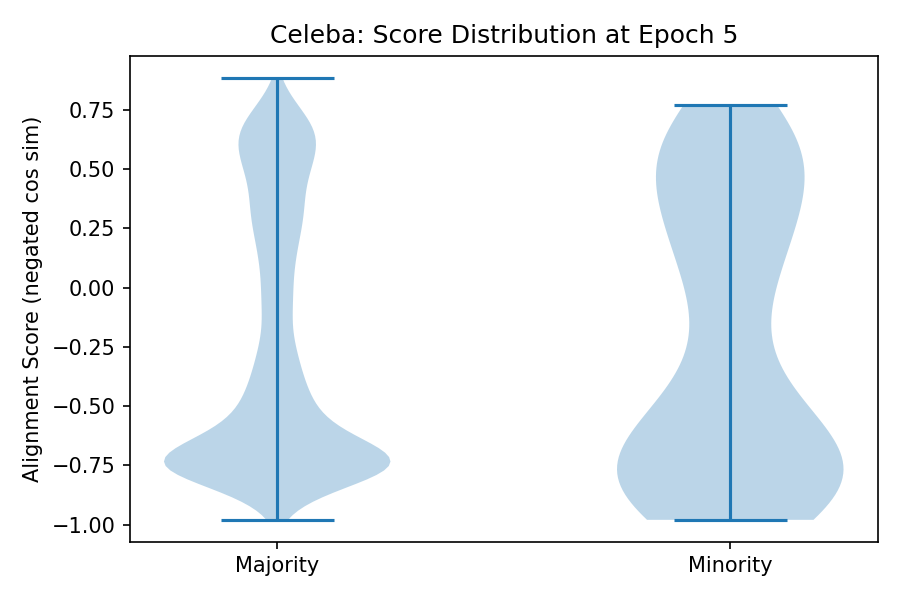
\includegraphics[width=\columnwidth]{figures/score_distribution_epoch5_celeba.png}
\caption{Score distributions at epoch 5 by group, CelebA}
\label{fig:score_distribution_epoch5_celeba}
\end{figure}

\textbf{Figure 5:} Alignment score and per-sample loss distributions at epoch 5 by group on CelebA (blond-male minority, group ID 3, vs. all others). Minority and majority alignment score distributions are near-identical, confirming that the alignment signal is non-discriminative at epoch 5 (alignment ROC-AUC = 0.484). Loss distributions show clear separation consistent with loss ROC-AUC = 0.949. Source: \texttt{h-e1/figures/score\textbackslash \_distribution\textbackslash \_epoch5\textbackslash \_celeba.png}.

\subsubsection{B. ROC Curves at Best Alignment Epoch}

\begin{figure}[htbp]
\centering
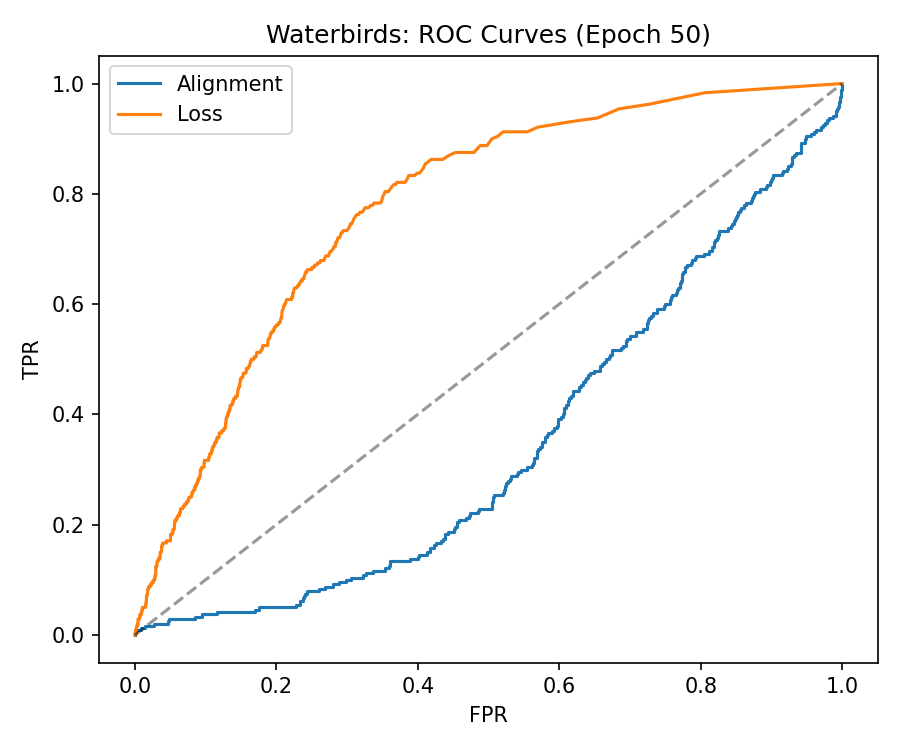
\includegraphics[width=\columnwidth]{figures/roc_curves_best_epoch_waterbirds.png}
\caption{ROC curves at epoch 50 (best alignment epoch), Waterbirds}
\label{fig:roc_curves_best_epoch_waterbirds}
\end{figure}

\textbf{Figure 6:} ROC curves at epoch 50 (the epoch at which alignment achieves its best performance on Waterbirds). The alignment ROC curve (AUC = 0.349) lies near the diagonal, indicating near-random discriminability; the loss ROC curve (AUC = 0.775) shows substantial area above the diagonal. Source: \texttt{h-e1/figures/roc\textbackslash \_curves\textbackslash \_best\textbackslash \_epoch\textbackslash \_waterbirds.png}.

\begin{figure}[htbp]
\centering
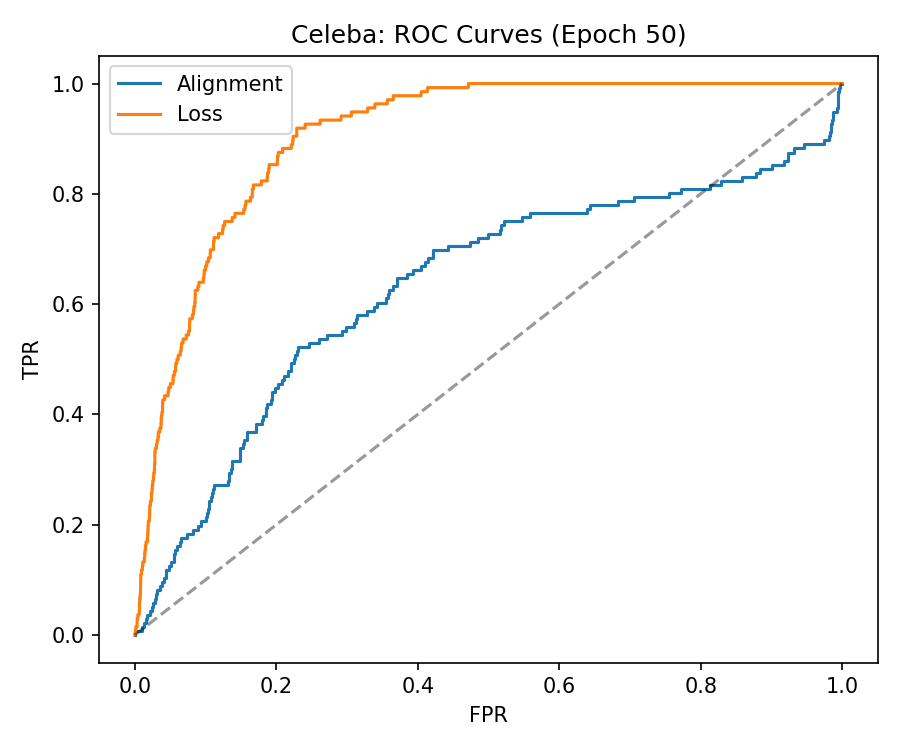
\includegraphics[width=\columnwidth]{figures/roc_curves_best_epoch_celeba.png}
\caption{ROC curves at epoch 50 (best alignment epoch), CelebA}
\label{fig:roc_curves_best_epoch_celeba}
\end{figure}

\textbf{Figure 7:} ROC curves at epoch 50 (the epoch at which alignment achieves its best performance on CelebA). Alignment ROC-AUC = 0.632, showing slightly positive but weak discriminability; loss ROC-AUC = 0.905. Source: \texttt{h-e1/figures/roc\textbackslash \_curves\textbackslash \_best\textbackslash \_epoch\textbackslash \_celeba.png}.

\subsubsection{C. Experiment Configuration Details}

Full experiment configuration, including minority group ID encoding and dataset preprocessing, is provided in Section 3 (Methodology). Raw numerical results at full precision are available in \texttt{h-e1/code/outputs/results.json} and \texttt{h-e1/experiment\textbackslash \_results.json}. Code is available at [anonymized for review].
